% !TEX encoding = UTF-8 Unicode
% !TEX TS-program = XeLaTeX
\documentclass[UTF8,12pt,letterpaper,oneside]{amsart}
\usepackage[letterpaper]{geometry}
\geometry{top=1.0in, bottom=1.0in, left=1.0in, right=1.0in}
\usepackage{setspace}
%\doublespacing
\usepackage{hyperref}
%\usepackage{times}
\usepackage{graphicx}
\usepackage{rotating}
\usepackage{multirow}
\usepackage{lineno} 
\usepackage{fancyhdr}
\usepackage{hanging}
\pagestyle{fancy}
\rhead{\textsc{Yang} \thepage} 
\renewcommand{\headrulewidth}{0pt} 
\renewcommand{\footrulewidth}{0pt} 
\setlength\headsep{0.333in}
\usepackage{tikz}
%\usepackage{shapes,backgrounds}

\newenvironment{workscited}{\newpage \begin{center} Works Cited \end{center}}{\newpage }

\begin{document}

\noindent Luke \textsc{Yang}\\
\texttt{1004-3383-46}\\
EE 101 TTh lecture\\
\textsc{Dr.} Satsuki \textsc{Takahashi}\\
Due Thursday, Feburary 13, 2014\\
Homework \#2\\

1.

a. 

\begin{tabular}{c|ccccc}
$ABC$ & $A^\prime$ & $B^\prime$ & $A^\prime + B^\prime$ & $C$ & $F$\\\hline
\texttt{000} & \texttt{1} & \texttt{1} & \texttt{1} & \texttt{0} & \texttt{0}\\\hline
\texttt{001} & \texttt{1} & \texttt{1} & \texttt{1} & \texttt{1} & \texttt{1}\\\hline
\texttt{010} & \texttt{1} & \texttt{0} & \texttt{1} & \texttt{0} & \texttt{0}\\\hline
\texttt{011} & \texttt{1} & \texttt{0} & \texttt{1} & \texttt{1} & \texttt{1}\\\hline
\texttt{100} & \texttt{0} & \texttt{1} & \texttt{1} & \texttt{0} & \texttt{0}\\\hline
\texttt{101} & \texttt{0} & \texttt{1} & \texttt{1} & \texttt{1} & \texttt{1}\\\hline
\texttt{110} & \texttt{0} & \texttt{0} & \texttt{0} & \texttt{0} & \texttt{0}\\\hline
\texttt{111} & \texttt{0} & \texttt{0} & \texttt{0} & \texttt{1} & \texttt{0}\\\hline
\end{tabular}

$F = A^\prime B^\prime C + A^\prime BC + AB^\prime C = m_1 + m_3 + m_5 = \sum_{ABC}(1, 3, 5)$

b.

\begin{tabular}{c|cccccc}
$WXY$ & $W^\prime$ & $X^\prime$ & $Y^\prime$ & $WX^\prime$ & $XY^\prime$ & $G$\\\hline
\texttt{000} & \texttt{1} & \texttt{1} & \texttt{1} & \texttt{0} & \texttt{0} & \texttt{1}\\\hline
\texttt{001} & \texttt{1} & \texttt{1} & \texttt{0} & \texttt{0} & \texttt{0} & \texttt{1}\\\hline
\texttt{010} & \texttt{1} & \texttt{0} & \texttt{1} & \texttt{0} & \texttt{1} & \texttt{1}\\\hline
\texttt{011} & \texttt{1} & \texttt{0} & \texttt{0} & \texttt{0} & \texttt{0} & \texttt{1}\\\hline
\texttt{100} & \texttt{0} & \texttt{1} & \texttt{1} & \texttt{1} & \texttt{0} & \texttt{1}\\\hline
\texttt{101} & \texttt{0} & \texttt{1} & \texttt{0} & \texttt{1} & \texttt{0} & \texttt{1}\\\hline
\texttt{110} & \texttt{0} & \texttt{0} & \texttt{1} & \texttt{0} & \texttt{1} & \texttt{1}\\\hline
\texttt{111} & \texttt{0} & \texttt{0} & \texttt{0} & \texttt{0} & \texttt{0} & \texttt{1}\\\hline
\end{tabular}

$G = W^\prime + X^\prime + Y^\prime = M_7 = \prod_{WXY}(7)$

2.\begin{equation*}\begin{split}
G =& \sum_{ABCD}(0, 2, 4, 6, 13, 15)\\
  =& A^\prime B^\prime C^\prime D^\prime + A^\prime B^\prime C D^\prime + A^\prime B C^\prime D^\prime + A^\prime BC D^\prime + AB C^\prime D + ABCD\\
  =& \prod_{ABCD}(1, 3, 5, 7, 8, 9, 10, 11, 12, 14)\\
  =& (A + B + C + D^\prime)(A + B + C^\prime + D^\prime)(A + B^\prime + C+ D^\prime)(A + B^\prime + C^\prime + D^\prime)\\&(A^\prime + B + C + D)(A^\prime + B + C + D^\prime)(A^\prime + B + C^\prime + D)(A^\prime + B + C^\prime + D^\prime)\\&(A^\prime + B^\prime + C + D)(A^\prime + B^\prime + C^\prime + D)
\end{split}\end{equation*}

4. a. \begin{equation*}\begin{split}
F &= X + [(W^\prime Y^\prime Z)(W + (X^\prime(Y + Z)))]\\
  &= X + [W^\prime Y^\prime Z(W + X^\prime Y + X^\prime Z)]\\
  &= X + [WW^\prime Y^\prime Z + W^\prime X^\prime YY^\prime Z + W^\prime X^\prime Y^\prime ZZ]\\
  &= X + [0 + 0 + W^\prime X^\prime Y^\prime Z]\\
  &= (X + W^\prime)(X + X^\prime)(X + Y^\prime)(X + Z)\\
  &= (X + W^\prime)(X + Y^\prime)(X + Z)
\end{split}\end{equation*}

b. \begin{equation*}\begin{split}
G &= AB + D(B^\prime + C)(A^\prime + C)\\
  &= AB + D(A^\prime B^\prime  + A^\prime C + B^\prime C + CC)\\
  &= AB + D(A^\prime B^\prime  + A^\prime C + B^\prime C + C)\\
  &= AB + D(A^\prime B^\prime  + C(A^\prime + B^\prime + 1))\\
  &= AB + D(A^\prime B^\prime  + C)\\
  &= AB + A^\prime B^\prime D  + CD
\end{split}\end{equation*}

5. \begin{equation*}\begin{split}
J &= P + R^\prime S\\
  &= (PRS + PR^\prime S + PRS^\prime + PR^\prime S^\prime) + (PR^\prime S + P^\prime R^\prime S)\\
  &= PRS + PR^\prime S + PRS^\prime + PR^\prime S^\prime + P^\prime R^\prime S\\
  &= m_7 + m_5 + m_6 + m_4 + m_1\\
  &= \sum_{WYZ}(1, 4, 5, 6, 7)
\end{split}\end{equation*}

6.

a. The faulty OR gate always outputs 1 even if it is supposed to output 0 and let H output 0, per the special input we give, which is the mechanism we use to identify the faulty OR gate. For the top gate, the combined input is \texttt{011}. For the middle gate, the combined input is \texttt{101}. For the bottom gate, the combined input is \texttt{010}.

b. No. In this case the final output (H) would always output 0 because it is an AND gate and always receives a 0 input from the faulty gate. No combination of input can make H change, thus we can't identify the faulty gate.

7.

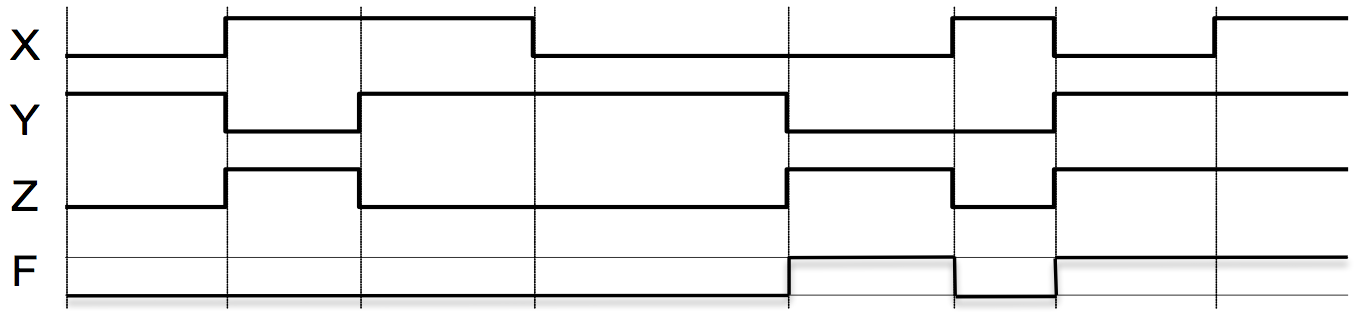
\includegraphics[scale=0.35]{hw2waveform.png}

8.

a. \begin{equation*}\begin{split}
G &= (A^\prime(BC)^\prime + (A^\prime + B^\prime))^\prime\\
  &= (A^\prime(BC)^\prime)^\prime (A^\prime + B^\prime)^\prime\\
  &= (A + BC)(AB)\\
  &= AAB + ABBC\\
  &= AB + ABC\\
  &= AB(1 + C)\\
  &= AB
\end{split}\end{equation*}

b. $G = AB = \sum_{AB}(3) = AB(C + C^\prime) = ABC + ABC^\prime = \sum_{ABC}(6, 7)$

9.

a.

\begin{tabular}{c|llll}
$C$/$AB$ & 00 & 01 & 11 & 10\\\hline
0 & ${}^0 1$ & ${}^2 1$ & ${}^6$ & ${}^4 1$\\\hline
1 & ${}^1$ & ${}^3$ & ${}^7 1$ & ${}^5$
\end{tabular}

SOP$ = A^\prime C^\prime + B^\prime C^\prime + ABC$

\begin{tabular}{c|llll}
$C$/$AB$ & 00 & 01 & 11 & 10\\\hline
0 & ${}^0$ & ${}^2$ & ${}^6 0$ & ${}^4$\\\hline
1 & ${}^1 0$ & ${}^3 0$ & ${}^7$ & ${}^5 0$
\end{tabular}

POS$ = (A + C^\prime)(B + C^\prime)(A^\prime + B^\prime + C)$

b.

\begin{tabular}{c|llll}
$YZ$/$WX$ & 00 & 01 & 11 & 10\\\hline
00 & ${}^0 1$ & ${}^4 1$ & ${}^{12}$ & ${}^8$\\\hline
01 & ${}^1 1$ & ${}^5 1$ & ${}^{13} 1$ & ${}^9 1$\\\hline
11 & ${}^4$ & ${}^7$ & ${}^{15}$ & ${}^{11}$\\\hline
10 & ${}^2$ & ${}^6 1$ & ${}^{14}$ & ${}^{10} 1$\\\hline
\end{tabular}

SOP$ = W^\prime Y^\prime + Y^\prime Z + W^\prime X Z^\prime + WX^\prime Y Z^\prime$

\begin{tabular}{c|llll}
$YZ$/$WX$ & 00 & 01 & 11 & 10\\\hline
00 & ${}^0$ & ${}^4$ & ${}^{12} 0$ & ${}^8 0$\\\hline
01 & ${}^1$ & ${}^5$ & ${}^{13}$ & ${}^9$\\\hline
11 & ${}^4 0$ & ${}^7 0$ & ${}^{15} 0$ & ${}^{11} 0$\\\hline
10 & ${}^2 0$ & ${}^6$ & ${}^{14} 0$ & ${}^{10}$\\\hline
\end{tabular}

POS$= (Y^\prime + Z^\prime)(W + X + Y^\prime)(W^\prime + X^\prime + Y^\prime)(W^\prime + Y + Z)$

10.

Note that
$A \oplus B = A^\prime B + AB^\prime = AA^\prime + AB^\prime + A^\prime B + BB^\prime = (A + B)(A^\prime + B^\prime) = (A + B)(AB)^\prime$,


the result of the revised circuit,

\begin{equation*}\begin{split}
Y &= [([(A + B)^\prime + AB]^\prime C + AB)^\prime + ([D + E][DE]^\prime)^\prime]^\prime + DE\\
  &= ([(A + B)(AB)^\prime] C + AB)([D + E][DE]^\prime) + DE\\
  &= [(A \oplus B)C + AB](D \oplus E) + DE
\end{split}\end{equation*}

is exactly the same as the golden design.


\end{document}

